%\documentclass[12pt]{article}
%\usepackage[a4paper, margin=1in]{geometry} 
%\usepackage{graphicx} 
%\usepackage{hyperref}
%\usepackage{float}
%\usepackage{multicol}
%\usepackage{amsmath}
%\usepackage[ruled]{algorithm2e}
%\usepackage[font=small, labelfont=bf]{caption}
%
%\begin{document}

%
% Global alignment with DP
%
\subsection{Global alignment with DP}
Dynamic programming (DP) provides a solution for a multi-stage decision process, in which larger decisions recursively nest smaller decisions.

\subsubsection*{Memorize the best score in a table cell}

The most basic step of DP procedures is updatig a cell with the hightet score from the three different scores calculated from its adjacent cells. DP ends when all the table cells are updated.

\begin{figure}[H]
  \centering
      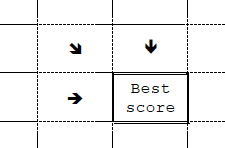
\includegraphics[width=0.25\textwidth]{fig02/dynamic_programmoing_cell_update.png}
\end{figure}

%
% Table notation and indices
%	
\subsubsection*{Table notation and indices}
$H_{i,j}$ represents the score of the cell for the current update. $H_{i-1,j}$, $H_{i,j-1}$,and $H_{i-1,j-1}$ are the scores of the adjacent cells.

\begin{multicols}{2}

Cell $H_{i, j}$ and its adjcent cells
\begin{figure}[H]
  \centering
      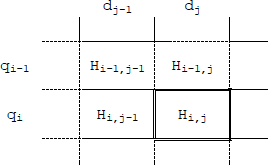
\includegraphics[width=0.3\textwidth]{fig02/dynamic_programmoing_cell_indices.png}
\end{figure}

Example
\begin{figure}[H]
  \centering
      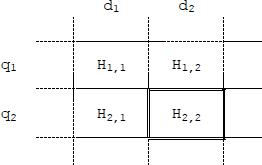
\includegraphics[width=0.3\textwidth]{fig02/dynamic_programmoing_cell_indices_example.png}
\end{figure}

\end{multicols} 

%
% Calculation of three candidate scores
%	
\subsubsection*{Calculation of three candidate scores}
$H_{i,j}^{(0)}$, $H_{i,j}^{(1)}$, and $H_{i,j}^{(2)}$ represent the three candidate scores of $H_{i,j}$. They are respectively calculated as:
\begin{align*}
H_{i,j}^{(0)} &= H_{i-1,j} - g &(vertical) \\
H_{i,j}^{(1)} &= H_{i,j-1} - g	&(horizontal) \\
H_{i,j}^{(2)} &= H_{i-1,j-1} + R_{a,b} &(diagonal)
\end{align*}

%
% Exercise \thesection.4
%
\subsubsection*{Exercise \thesection.4}

Calculate the scores of $H_{4,6}^{(0)}$, $H_{4,6}^{(1)}$, and $H_{4,6}^{(2)}$ first and then update $H_{4,6}$.
\begin{multicols}{2}
\begin{figure}[H]
  \centering
      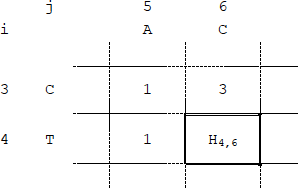
\includegraphics[width=0.3\textwidth]{fig02/dynamic_programmoing_cell_update_exercise.png}
\end{figure}

\noindent Scoring scheme: \\ 
$R_{ab}$ = 1 for a = b \\ 
$R_{ab}$ = 0 for a $\neq$ b \\ 
g = 1

\end{multicols} 

%
% Initialization
%
\subsubsection*{Initialization}

The first row and the first column can be calcuated independently from the adjcent cells.
\begin{align*}
H_{0,j} &:  j * -1 * g \\
H_{i,0} &: i * -1 * g
\end{align*}

\noindent
Example
\begin{figure}[H]
  \centering
      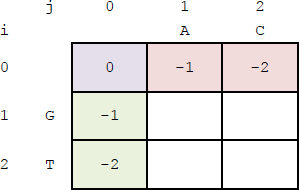
\includegraphics[width=0.3\textwidth]{fig02/dynamic_programmoing_initialization.png}
\end{figure}

%
% Exercise \thesection.5
%
\subsubsection*{Exercise \thesection.5}
Update all cells of Table 1 and 2. Use the scoring scheme in Exercise \thesection.4.

\begin{multicols}{2}
Table 1
\begin{figure}[H]
  \centering
      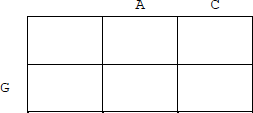
\includegraphics[width=0.3\textwidth]{fig02/global_alignment_exercise1.png}
\end{figure}

\vfill\null
\columnbreak

Table 2
\begin{figure}[H]
  \centering
      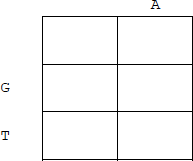
\includegraphics[width=0.25\textwidth]{fig02/global_alignment_exercise2.png}
\end{figure}

\end{multicols} 

%
% Sub-solutions
%
\subsubsection*{Sub-solutions}

In DP, larger decisions recursively nest smaller decisions. For instance, Table S is included in Table L.

\begin{multicols}{2}
Table S
\begin{figure}[H]
  \centering
      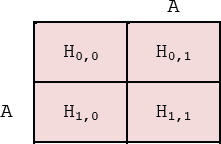
\includegraphics[width=0.3\textwidth]{fig02/dynamic_programmoing_subsolution_S.png}
\end{figure}

\vfill\null
\columnbreak

Table L
\begin{figure}[H]
  \centering
      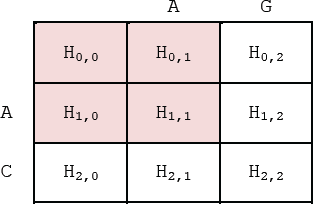
\includegraphics[width=0.4\textwidth]{fig02/dynamic_programmoing_subsolution_L.png}
\end{figure}

\end{multicols} 

%
% NEW PAGE
%
\newpage

%
% Psedo-code of global alignment with DP
%
\subsubsection*{Psedo-code of updating DP table for global alignment}

\begin{algorithm}[H]
  \SetKwInOut{HAB}{$\mathrm{H_{i,j}}$}
  \SetKwInOut{RAB}{$\mathrm{R_{a,b}}$}
  \SetKwInOut{G}{$\mathrm{g}$}
  \SetKwData{dRAB}{$\mathrm{R_{a,b}}$}
  \SetKwData{dG}{$\mathrm{g}$}
  
  \BlankLine
    
  \HAB{Dyanamic programming table}
  \RAB{Match/mismatch scores}
  \G{Gap penalty}
  
  \BlankLine \BlankLine
  
  \tcp{Initialization}
  \For{$i \leftarrow 0$ \KwTo $m$}{
    $\mathrm{H_{i,0}}$ $\leftarrow$ $i * -1 * g$\;
  }
  \For{$j \leftarrow 1$ \KwTo $n$}{
    $\mathrm{H_{0,j}}$ $\leftarrow$ $j * - 1 * g$\;
  }
  
  \BlankLine \BlankLine
    
  \tcp{Main loop for table update}
  \For{$i \leftarrow 1$ \KwTo $m$}{
    \For{$j \leftarrow 1$ \KwTo $n$}{
      $\mathrm{H_{i,j}}$ $\leftarrow$ $max(\mathrm{H_{i-1,j}} - \dG, \mathrm{H_{i,j-1}} - \dG, \mathrm{H_{i-1,j-1}}$ + \dRAB)\;
    }
  }
  
  \SetAlgoRefName{\thesection.1}
  \caption{Update dynamic programming table for global alignment}

\end{algorithm}

%\end{document}
